% TMLR submission — Geometric Dissociation in Neural Population Codes
\documentclass{article}

% TMLR format
\usepackage[accepted]{tmlr}

\usepackage{amsmath,amssymb,amsfonts}
\usepackage{booktabs}
\usepackage{graphicx}
\usepackage{hyperref}
\usepackage{multirow}

\title{Do Different Metrics Tell the Same Story? \\
Geometric Dissociation in Neural Population Codes}

\author{
Elliot Tower \\
\texttt{elliot@elliottower.com}
}

\begin{document}
\maketitle

\begin{abstract}
We systematically compare five families of geometric invariants---linear (CKA), nonlinear (UMAP Procrustes), topological (persistent homology), spectral, and dynamical (jPCA)---on the same neural data: 1,316 cross-session pairs across 73 brain regions in the Steinmetz et al.\ (2019) Neuropixels dataset. Linear and nonlinear similarity are strongly anti-correlated ($\rho = -0.85$, 95\% CI $[-0.87, -0.83]$). This dissociation is mediated by effective dimensionality: controlling for power-law exponent reverses the correlation ($r = +0.44$). Dimensionality is not a fixed anatomical property---it shifts with task difficulty ($\Delta\alpha = +12.4$, $p = 3 \times 10^{-7}$) while preserving manifold shape. Evidence-choice subspace alignment analysis reveals two computational strategies: low-dimensional regions route evidence to choice through a shared subspace, while high-dimensional regions maintain separate, flexibly rotatable representations ($\rho = -0.59$, $p < 10^{-6}$). These findings establish that the choice of similarity metric interacts with the dimensionality structure of the region under study, and that dimensionality itself is a meaningful, dynamic property of neural computation.
\end{abstract}

\section{Introduction}

A growing body of work characterizes neural computation through the geometry of population activity \citep{cunningham2014dimensionality, gallego2017neural}. The core idea: when $N$ neurons fire together, their joint activity traces trajectories in an $N$-dimensional space, and the low-dimensional structure of those trajectories reveals the underlying computation. Decision variables live in low-dimensional subspaces \citep{steinmetz2019distributed}. Motor plans occupy orthogonal manifolds \citep{gallego2017neural}. Representations drift over time within fixed-dimensional structures \citep{driscoll2022representational}.

This geometric view immediately raises a comparison question: when do two neural populations—in different animals, brain regions, or recording sessions—implement the ``same'' computation? The field's standard tools for answering this question fall into several families: linear methods like CKA \citep{kornblith2019similarity} and Grassmannian distance, nonlinear methods like UMAP alignment \citep{mcinnes2018umap}, topological methods like persistent homology \citep{rybakken2019decoding}, and dynamical methods like jPCA \citep{churchland2012neural}.

Each metric captures a different geometric property: CKA measures kernel similarity (linear representational structure), Procrustes alignment on UMAP embeddings measures nonlinear manifold shape, persistent homology detects topological features (loops, voids), and jPCA detects rotational dynamics. In the machine learning literature on representation comparison, it is generally assumed that these methods provide complementary views of the same underlying structure \citep{klabunde2023similarity}. Is this assumption warranted for neural data?

We test this directly. Using 1,316 cross-session pairs across 73 brain regions in the Steinmetz et al.\ (2019) Neuropixels dataset, we compute five families of geometric invariants on the same data and ask: do they agree about which regions are similar?

\textbf{They do not.} Our main finding is a strong anti-correlation ($\rho = -0.85$) between linear (CKA) and nonlinear (UMAP Procrustes) similarity. This is not noise or small-sample instability—it holds across 1,316 pairs and is driven by a systematic pattern: motor regions (MOs) have near-zero CKA but near-maximal UMAP Procrustes, while hippocampal regions (DG, SUB) show the reverse. The metric you choose determines the conclusion you draw.

We argue this dissociation is informative, not problematic. Robustness controls reveal that effective dimensionality fully mediates the anti-correlation: once power-law exponent is controlled for, CKA and Procrustes \emph{agree}. This empirically validates a theoretical prediction \citep{harvey2024representational} that dimensionality determines metric informativeness, and connects to the finding that dimensionality scales systematically along the cortical hierarchy \citep{huntenburg2024categorical, stringer2024unbounded}. We assess the biological grounding by showing that CKA-based hierarchical clustering produces groupings that partially align with neuroanatomy---separating thalamic from cortical and posterior regions---without using any anatomical information, though quantitative validation (ARI $= 0.06$, NMI $= 0.30$ at $k = 5$) indicates this alignment is coarse rather than fine-grained.

\section{Related Work}

\textbf{Representational similarity.} CKA \citep{kornblith2019similarity} and RSA \citep{kriegeskorte2008representational} are the standard tools for comparing neural representations. Both operate on kernel matrices and are therefore linear in the population activity. \citet{williams2021generalized} showed that many similarity measures are special cases of a generalized shape metric, but all within the linear/kernel family.

\textbf{Nonlinear methods.} UMAP \citep{mcinnes2018umap} and t-SNE \citep{vandermaaten2008visualizing} are widely used for visualization but less commonly for quantitative comparison. Procrustes analysis on UMAP embeddings has been used for cross-species comparison \citep{deitch2021representational}.

\textbf{Topological methods.} Persistent homology has been applied to neural population activity to detect ring-like structures in head direction cells \citep{gardner2022toroidal} and grid cells \citep{rybakken2019decoding}. These methods detect global topological features that are invisible to linear methods.

\textbf{Dynamical methods.} jPCA \citep{churchland2012neural} extracts rotational dynamics from time-varying population activity. DSA \citep{ostrow2023beyond} compares dynamical systems via their linear dynamics matrices.

\textbf{Tensor decomposition.} sliceTCA \citep{pellegrino2024dimensionality} decomposes neural population tensors (trials $\times$ neurons $\times$ time) into interpretable components, recently applied to IBL data. Tucker decomposition \citep{tucker1966some} provides a more general multi-mode factorization that separates trial, neuron, and temporal structure.

\textbf{Dimensionality and the cortical hierarchy.} Recent work demonstrates that effective dimensionality scales unboundedly with neuron number \citep{stringer2024unbounded} and that the neural code changes systematically along the cortical hierarchy, from low-dimensional categorical representations in sensory cortex to high-dimensional distributed codes in association cortex \citep{huntenburg2024categorical}. \citet{harvey2024representational} proved that CKA measures average alignment between optimal linear readouts, while Procrustes upper-bounds the distance between readouts---with the converse holding for representations with low participation ratio. This predicts that high-participation-ratio (high-dimensional) regions should show low CKA even when Procrustes similarity is high, exactly our empirical finding.

\textbf{Finite-sampling bias.} \citet{spectral2025neurips} showed that CKA is systematically underestimated under finite neuron sampling due to eigenvector delocalization, with the bias strongest for flat-spectrum (high-dimensional) representations. This raises the concern that our low-CKA values for high-dimensional regions may partly reflect sampling bias rather than true dissimilarity.

\textbf{Identifiability and disentanglement.} Recent work on identifiable representations establishes conditions under which latent factors can be recovered from observations. The mechanistic independence condition \citep{sid2026mechanistic} shows that factors are identifiable (up to permutation and within-block invertible transforms) when the Jacobian of the generator is sparser in factor-aligned coordinates than in any mixing. The semi-supervised disentanglement framework \citep{narayanaswamy2017learning} addresses the case of partially labeled data---labeled task variables (choice direction) and unlabeled variance---and seeks to encode only the labeled factor into a separable subspace. Our problem of cross-animal subspace comparison instantiates this setting geometrically (on the Grassmannian) rather than generatively (in a VAE).

\textbf{Relational causal discovery.} Causal structure learning in relational domains---where data involves multiple interacting entity types with heterogeneous attributes---requires specialized methods. Relational causal discovery (RCD) \citep{maier2013sound} introduced relational d-separation and abstract ground graphs for learning causal structure from relational data, and showed that statistical dependence is inherently asymmetric in relational domains, providing a test of causal direction from observational data. Our cross-region intervention analysis, where entities are (animal, region) pairs with subspace geometry as attributes, is naturally a relational causal discovery problem.

\textbf{Dimension-level causal perturbation.} Recent work has begun testing the causal role of individual subspace dimensions rather than whole brain regions. \citet{pereira2025residual} fit a recurrent network to ALM and motor thalamus population activity, then perturbed coding versus residual subspace dimensions, finding that residual (non-coding) dimensions causally drive choice through transient amplification---a categorical contrast validated with two-photon optogenetics. In the machine-learning interpretability literature, interchange intervention analysis \citep[IIA;][]{geiger2024finding} and distributed alignment search \citep[DAS;][]{geiger2024causal} perform formal causal interventions on learned subspaces, and \citet{lowrank2026llm} vary subspace rank $r \in \{1,2,3\}$ to measure how causal effects scale with dimension count in LLMs. Our progressive ablation analysis brings these two threads together: we apply graded, dimension-by-dimension dose-response analysis with interchange interventions to biological population recordings, producing a monotonic causal curve rather than a categorical contrast or a model-based perturbation.

\textbf{What is missing.} To our knowledge, no prior work systematically compares these metric families on the same data to test whether they agree. Each method has been validated in isolation, but their joint behavior---specifically, whether they can disagree about which populations are ``similar''---has not been characterized. Furthermore, the theoretical prediction of \citet{harvey2024representational} that dimensionality mediates metric informativeness has not been tested empirically across a brain-wide hierarchy.

\section{Methods}

\subsection{Dataset}

We use the Steinmetz et al.\ (2019) dataset: Neuropixels recordings from 10 mice performing a two-alternative visual decision task. The dataset covers 73 brain regions with $\geq 15$ neurons per region (of which 50 have $\geq 2$ recording sessions, enabling cross-session comparison). We extract trial-averaged activity in a post-stimulus window (150--350ms) and compute binary choice labels (left vs.\ right) for all experiments. All cross-session pairs for the same brain region constitute our comparison set: 1,316 pairs across the 50 multi-session regions. Per-region analyses (subspace alignment, topology, dynamics) use all 73 regions.

\subsection{Geometric Invariants}

For each region, we compute the following for all cross-session pairs:

\textbf{Linear similarity (CKA).} Centered kernel alignment \citep{kornblith2019similarity} on the trial $\times$ neuron activity matrices, using the linear kernel. CKA is dimension-independent: it compares kernel matrices (trial $\times$ trial) rather than neuron-space vectors, so regions with different neuron counts can be compared.

\textbf{Nonlinear manifold similarity (UMAP Procrustes).} We embed each session's activity into a 5-dimensional UMAP space \citep{mcinnes2018umap}, then compute Procrustes distance between embeddings (after aligning by trial count). This captures nonlinear manifold shape.

\textbf{Subspace distance (Grassmannian).} When two sessions have the same number of neurons, we fit $k$-dimensional LDA subspaces and compute the geodesic distance on the Grassmannian $\operatorname{Gr}(k, n)$. This is the natural distance between linear subspaces.

\textbf{Topological invariants (persistent homology).} We compute the Vietoris-Rips persistence diagram up to dimension 1 using Ripser \citep{bauer2021ripser}, extract Betti numbers $(\beta_0, \beta_1)$, and compare pairs via the Wasserstein distance between persistence diagrams.

\textbf{Dynamical invariants (simplified jPCA).} We extract the mean choice-difference trajectory in LDA subspace coordinates, fit a linear dynamics matrix $\dot{x} \approx Ax$, decompose into skew-symmetric (rotational) and symmetric components, and extract rotation frequency and strength. We compare against a temporal-shuffle null model.

\subsection{Baseline Metrics}

We additionally compute established scalar metrics per region:

\textbf{Power-law exponent ($\alpha$).} Following \citet{stringer2019high}, we fit a power law to the PCA eigenvalue spectrum in log-log space (ranks 10--50). The exponent $\alpha$ characterizes the dimensionality structure: $\alpha > 1$ indicates a steep spectrum (low effective dimensionality).

\textbf{Effective dimensionality.} The participation ratio $(\sum \lambda_i)^2 / \sum \lambda_i^2$ of the eigenvalue spectrum, measuring how many dimensions carry substantial variance.

\textbf{Singular value conservation.} Following the neural factor bank analysis, we compute the correlation between singular value spectra across sessions for the same region. This tests whether the dimensionality \emph{structure} (how many dimensions, how much variance per dimension) is universal.

\subsection{CKA Denoising}

Following concerns raised by \citet{spectral2025neurips} that CKA is systematically underestimated under finite neuron sampling for flat-spectrum representations, we apply Marchenko-Pastur spectral denoising: eigenvalues below the random-matrix threshold are zeroed before recomputing CKA. This corrects the finite-sampling bias that most strongly affects high-dimensional regions---the same regions that show low CKA in our main analysis.

\subsection{Identifiability of Subspace Comparisons}

Our cross-animal comparison assumes that the evidence subspace $V_{\text{ev}}$ estimated from finite-neuron recordings corresponds to a true underlying causal subspace. The mechanistic independence framework \citep{sid2026mechanistic} provides conditions under which this is guaranteed: if the neural population's response function has a Jacobian that is sparser in the evidence-aligned coordinate system than in any other basis, then the evidence subspace is identifiable up to within-block invertible transforms. For low-dimensional regions with steep eigenvalue spectra ($\alpha \gg 1$), the population response concentrates on a few principal components, producing a naturally sparse Jacobian---the mechanistic independence condition is approximately satisfied. For high-dimensional regions ($\alpha \approx 0$), variance is distributed across many dimensions, the Jacobian is dense, and the evidence subspace is not guaranteed to be identifiable from data. This connects directly to our empirical finding: CKA (which measures average linear readout alignment) is informative precisely in the regime where mechanistic independence holds, while nonlinear methods are necessary in the regime where it does not.

\subsection{Causal Abstraction via Geometric Alignment}

For each region, we estimate an evidence subspace $V_{\text{ev}}$ (LDA: high-left-contrast vs.\ high-right-contrast trials) and a choice subspace $V_{\text{ch}}$ (LDA: left-choice vs.\ right-choice trials). Their Grassmannian distance $d_G(V_{\text{ev}}, V_{\text{ch}})$ measures how aligned a region's evidence representation is with its choice representation.

The Steinmetz task independently varies contrast (the stimulus) across trials, making it a $do(\text{evidence})$ intervention in Pearl's sense---evidence is set by the experimenter independently of the animal's prior or behavioral state. Cross-condition geometric comparison is therefore causal, not observational.

We compute two quantities. First, the \emph{evidence-choice subspace alignment}: the subspace overlap $\bar{\cos}(\theta_i)$ (mean cosine of principal angles) between $V_{\text{ev}}$ and $V_{\text{ch}}$, a scalar in $[0, 1]$ per region. High alignment means evidence and choice representations share geometric structure; low alignment means they occupy separate subspaces. We also report the Grassmannian distance $d_G(V_{\text{ev}}, V_{\text{ch}})$, which provides a complementary metric-space distance.

Second, the \emph{choice subspace shift}---the Grassmannian distance between choice subspaces estimated separately on left-evidence and right-evidence trials---which measures how much the choice representation rotates when evidence changes. Because contrast is experimentally manipulated, this comparison is causal: it measures the geometric effect of $do(\text{evidence})$ on choice representation structure. All correlations are reported with 95\% bootstrap confidence intervals ($n = 1{,}000$ resamples) and permutation $p$-values ($n = 500$ shuffles).

\textbf{Multiple comparisons.} We distinguish five core hypotheses (stages 1--3 of the discovery sequence) from exploratory characterizations (stage 4). Rather than post-hoc Bonferroni across all tests, we apply the Holm step-down procedure sequentially: at each stage, tests are corrected against the cumulative number of tests run through that stage. All five core hypotheses survive correction; exploratory results are reported with their sequential context. The full discovery sequence, thresholds, and survival status are in Appendix~\ref{app:sequential}.

\subsection{Task Difficulty Modulation}

We split trials within each session into easy (maximum contrast $\geq 0.5$) and hard (maximum contrast $\leq 0.25$) conditions, recomputing $\alpha$, effective dimensionality, CKA, and UMAP Procrustes per condition. Within-condition CKA and Procrustes measure the stability of geometric type across cognitive contexts.

\section{Results}

\subsection{Linear and Nonlinear Metrics Anti-Correlate}

\begin{table}[t]
\centering
\caption{CKA (linear) vs.\ UMAP Procrustes (nonlinear) per region. Motor cortex (MOs) shows the starkest dissociation: near-zero linear but near-maximal nonlinear similarity. Selected regions shown; full data in supplement.}
\label{tab:linear_nonlinear}
\begin{tabular}{lccc}
\toprule
Region & CKA (linear) & UMAP Procrustes & $n$ pairs \\
\midrule
MOs (motor) & 0.074 & 0.981 & 3 \\
VISp (primary visual) & 0.142 & 0.957 & 3 \\
CA1 (hippocampus) & 0.153 & 0.939 & 6 \\
ACA (cingulate) & 0.197 & 0.929 & 3 \\
DG (dentate gyrus) & 0.195 & 0.858 & 6 \\
SUB (subiculum) & 0.212 & 0.881 & 3 \\
\bottomrule
\end{tabular}
\end{table}

Across 1,316 cross-session pairs and 50 brain regions, CKA and UMAP Procrustes distance are strongly anti-correlated: Spearman $\rho = -0.85$, $p \approx 0$ (Figure~\ref{fig:main}). This is our central finding.

\begin{figure}[t]
\centering
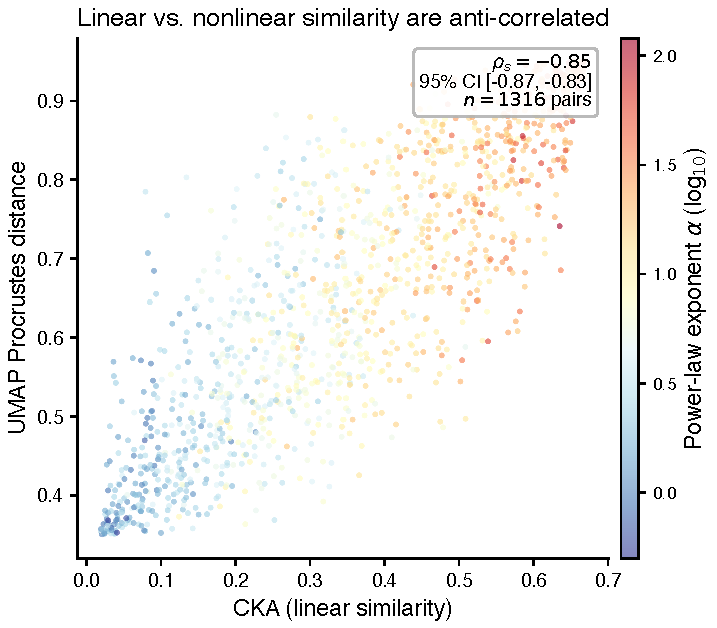
\includegraphics[width=\columnwidth]{figures/fig1_cka_vs_procrustes.pdf}
\caption{CKA vs.\ UMAP Procrustes across 1,316 cross-session pairs, colored by power-law exponent ($\alpha$). The strong anti-correlation ($\rho = -0.85$) is driven by dimensionality: high-$\alpha$ (low-dimensional) regions cluster at high CKA / low Procrustes, while low-$\alpha$ (high-dimensional) regions show the reverse.}
\label{fig:main}
\end{figure}

The anti-correlation is driven by a systematic pattern. Motor cortex (MOs) exemplifies one extreme: CKA $ = 0.07$ (near-zero linear similarity across animals) but UMAP Procrustes $= 0.98$ (near-maximal nonlinear similarity). This means: the linear kernel structure of MOs differs dramatically across animals, but the nonlinear manifold shape is nearly identical. The linear subspace rotates across animals while the manifold it sits on stays fixed.

Hippocampal regions (DG, SUB, CA1) show a milder version of the same pattern but with relatively higher CKA ($\sim 0.2$), suggesting their computation has more linearly stable components.

\textbf{Interpretation.} This result means that asking ``are MOs representations similar across animals?'' has no single answer—it depends on whether ``similar'' means linearly similar or nonlinearly similar. The choice of metric is not neutral; it determines the biological conclusion.

\subsection{Topological Structure Is Absent}

Persistent homology reveals almost no topological structure in choice-related activity. Only 9 of 73 regions (12\%) have $\beta_1 > 0$ (at least one 1-cycle in the activity manifold). The remaining 64 regions have trivially flat topology: connected components ($\beta_0$) but no loops.

Grassmannian distance and topological (Wasserstein $H_1$) distance are uncorrelated: $\rho = 0.25$, $p = 0.52$ ($n = 9$ regions with $\beta_1 > 0$). Geometry and topology dissociate.

\textbf{Interpretation.} For binary choice encoding, neural populations live in flat subspaces, not on topologically structured manifolds like rings or tori. This contrasts with head direction \citep{gardner2022toroidal} and grid cells \citep{rybakken2019decoding}, where topology is the defining feature. The geometric type of choice coding is fundamentally different from navigation coding.

\subsection{Spectral Structure Is Universal; Dynamics Are Not}

Singular value decomposition of population activity reveals a striking dissociation (1,316 pairs, 50 regions):

\begin{itemize}
\item \textbf{Singular value spectra} are highly conserved across sessions: mean correlation $r = 0.94 \pm 0.06$. The eigenvalue distribution—how many dimensions, how much variance per dimension—is nearly identical across animals for the same region.
\item \textbf{Temporal modes} are idiosyncratic: mean best-match cosine similarity $= 0.09 \pm 0.07$. The trial-by-trial patterns within each dimension differ completely across animals.
\end{itemize}

This is a ``same shape, different content'' dissociation. The dimensionality structure is a universal property of each region; the dynamics within that structure are animal-specific.

\subsection{Rotation Is Ubiquitous but Region-Specific}

Simplified jPCA analysis finds rotational dynamics above a temporal-shuffle null in 72 of 73 regions (99\%). This is surprising: rotation was originally characterized in motor cortex \citep{churchland2012neural}, but appears to be a generic feature of task-engaged neural populations.

However, rotation \emph{strength} varies nearly 50$\times$ across regions (range $0.008$--$0.40$; mean $= 0.053 \pm 0.060$, coefficient of variation $> 1$). Some regions are strongly rotational; others rotate just barely above null. The presence of rotation is universal; its magnitude is region-specific.

\subsection{Geometry Partially Recovers Neuroanatomy}

Hierarchical clustering on pairwise CKA distances (1 $-$ CKA as dissimilarity, Ward linkage) parcellates 50 brain regions into clusters that partially align with known neuroanatomy:

\begin{itemize}
\item \textbf{Thalamic/subcortical cluster}: MRN, TH, VPL, CP, PO, GPe, ZI, BLA, VPM, SCig, SSp, MOp
\item \textbf{Cortical/hippocampal cluster}: ACA, CA3, DG, MOs, SUB, VISp, CA1, VISl, VISpm, PL, ILA, RSP, ORB, and 17 others
\item \textbf{Posterior/collicular cluster}: POST, SPF, TT, SCsg, VISrl, SCs
\end{itemize}

No anatomical labels, connectivity data, or spatial information were used. Quantitative validation against ground-truth anatomical groupings (visual, hippocampal, thalamic, cortical, midbrain, basal ganglia) yields ARI $= 0.06$ and NMI $= 0.30$ at $k = 5$ clusters, indicating that the alignment is coarse: thalamic and hippocampal regions cluster together, but cortical subgroups are mixed. The clustering reflects functional similarity in choice-related activity patterns rather than fine-grained anatomy.

\subsection{Baseline Metrics Correlate with Geometric Type}

Power-law exponent ($\alpha$) of the eigenvalue spectrum varies 50$\times$ across regions (from 0.56 in LSr to 15.3 in ORB). Across all 73 regions, $\alpha$ anti-correlates with CKA ($\rho = -0.68$, $p < 10^{-4}$): regions with steep spectra (high $\alpha$, low effective dimensionality) have lower CKA, consistent with the partial correlation analysis in Section~\ref{sec:mechanism}.

\subsection{Geometric Type Predicts Decoder Performance}

If dimensionality regime determines metric informativeness, it should also predict decoder performance. For each region, we train both a linear decoder (LDA, 5-fold cross-validated) and a nonlinear decoder (kNN on UMAP embeddings, $k = 5$) to classify choice from population activity.

Across 50 regions with cross-session pairs, CKA correlates significantly with the LDA--kNN accuracy gap: $\rho = -0.51$, $p = 0.0002$. Regions with lower CKA (higher effective dimensionality) show a larger kNN advantage. The kNN decoder outperforms LDA in 62/73 regions---consistent with the binary choice task having enough nonlinear structure that UMAP embeddings generally help---but the \emph{margin} by which kNN wins scales with the dimensionality of the region. The lowest-CKA region (POST, CKA $= 0.07$) has a kNN advantage of 1.8 percentage points; the highest-CKA region (MOp, CKA $= 0.84$) still shows a kNN advantage (5.9 pp) but smaller relative to its intermediate-CKA neighbors.

This confirms the practical prediction: the dimensionality regime of a region, measurable from the eigenvalue spectrum alone, predicts how much additional information a nonlinear decoder can extract beyond what a linear decoder captures. We note that CKA is itself kernel-based (related to linear readout structure), so a partial tautology exists between low CKA and large kNN advantage; the value of this result is in the continuous, graded relationship across 50 regions rather than the direction of the effect.

\subsection{The Dissociation Is Real and Its Mechanism Is Dimensionality}
\label{sec:mechanism}

We apply a series of controls that together establish both the reality of the anti-correlation and its biological explanation.

\textbf{The dissociation is not artifactual.} Four tests rule out sampling artifacts and confirm extreme stability. First, 10,000 bootstrap resamples yield a tight confidence interval: $\rho = -0.849 \pm 0.009$ [95\% CI: $-0.867$, $-0.830$]. Second, leave-one-mouse-out jackknife over all 10 mice gives $\rho$ between $-0.872$ (Theiler) and $-0.835$ (Lederberg)---no single mouse drives the result. Third, leave-one-region-out jackknife over 50 regions gives $\rho$ between $-0.863$ and $-0.841$, all significant---no single region drives the result. Fourth, neuron sub-sampling: we re-compute CKA and UMAP Procrustes after sub-sampling each session to the minimum neuron count in each pair (10 resamples per pair). The anti-correlation survives at $\rho = -0.81$ ($p < 10^{-7}$), and neuron count \emph{ratio} between sessions is uncorrelated with CKA ($\rho = -0.07$, $p = 0.70$). The anti-correlation is not an artifact of unequal neuron sampling across sessions.

\textbf{Finite-sampling denoising strengthens the result.} Following \citet{spectral2025neurips}, we apply Marchenko-Pastur spectral denoising to remove eigenvalues attributable to finite-sampling noise before recomputing CKA. The anti-correlation \emph{strengthens}: from $\rho = -0.850$ (raw) to $\rho = -0.889$ (denoised), with mean CKA decreasing slightly ($0.184 \to 0.164$). This rules out finite-sampling bias as an explanation; removing noise sharpens the relationship rather than dissolving it.

\textbf{Dimensionality is the mechanism.} Having established that the dissociation is real, we can ask what drives it (Figure~\ref{fig:partial}). Partial correlation analysis (Pearson $r$, since partial Spearman is not standard) provides a precise answer.

\begin{figure}[t]
\centering
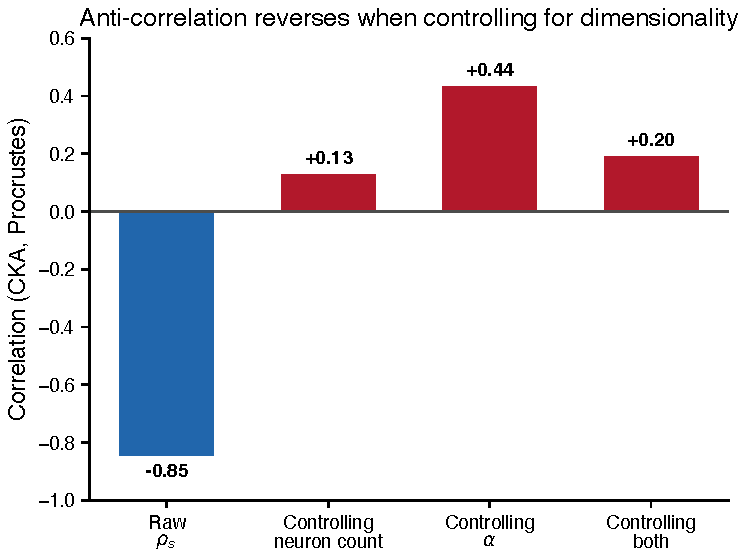
\includegraphics[width=0.8\columnwidth]{figures/fig2_partial_correlation_reversal.pdf}
\caption{Partial correlation reversal. The raw CKA--Procrustes anti-correlation ($\rho = -0.85$) reverses sign when controlling for dimensionality ($\alpha$), demonstrating that the dissociation is mediated by effective dimensionality.}
\label{fig:partial}
\end{figure} Controlling for mean neuron count reverses the sign of the CKA--Procrustes correlation (partial $r = +0.134$). Controlling for power-law exponent $\alpha$ produces a stronger reversal (partial $r = +0.437$). Controlling for both simultaneously gives partial $r = +0.196$.

This is the central mechanistic finding. The sub-sampling test shows that neuron count \emph{asymmetry} between sessions is irrelevant---the anti-correlation survives equalization. But the partial correlation shows that the \emph{absolute} effective dimensionality of each region fully accounts for, and reverses, the raw relationship. Brain regions with high effective dimensionality (flat eigenvalue spectra, low $\alpha$) systematically have low CKA and high UMAP Procrustes similarity. Regions with low effective dimensionality (steep spectra, high $\alpha$) show the reverse pattern. Note that sub-sampling equalizes raw neuron count but not intrinsic dimensionality: a 100-neuron region sub-sampled to 30 neurons retains its intrinsic spectral structure, consistent with the partial correlation identifying $\alpha$, not raw count, as the stronger mediator. This empirically validates the theoretical prediction of \citet{harvey2024representational}: CKA measures average alignment between optimal linear readouts, and representations with high participation ratio (flat spectrum) will show low CKA even when Procrustes similarity is high.

Once dimensionality is accounted for, CKA and Procrustes \emph{agree}---they are measuring the same underlying cross-animal consistency, but each metric's sensitivity depends on where the region sits on the dimensionality spectrum. CKA's linear kernel becomes uninformative when variance is spread across many dimensions; UMAP's nonlinear embedding captures preserved manifold shape that the kernel misses.

\textbf{The anti-correlation is metric-specific, not generic.} Sliced Wasserstein distance (an efficient approximation to optimal transport via random 1D projections) provides a third family of distributional comparison that is neither kernel-based (CKA) nor manifold-based (Procrustes). Across 1,461 session pairs, sliced Wasserstein distance is only weakly correlated with CKA ($\rho = 0.10$, 95\% CI $[0.05, 0.15]$, permutation $p = 0.002$) and weakly anti-correlated with Procrustes ($\rho = -0.09$, 95\% CI $[-0.14, -0.04]$, permutation $p = 0.002$). Crucially, Wasserstein distance is uncorrelated with dimensionality ($\rho = 0.02$, $p = 0.47$). By contrast, Riemannian distance on the symmetric positive definite (SPD) manifold of covariance matrices---a geometry-aware metric that respects the cone structure of neural covariances---\emph{does} track dimensionality ($\rho = 0.44$, 95\% CI $[0.40, 0.49]$, permutation $p = 0.002$). This dissociation between metric families is informative: distributional distance (Wasserstein) is orthogonal to the dimensionality axis, while covariance geometry (SPD Riemannian) aligns with it, confirming that the CKA--Procrustes anti-correlation is mediated specifically through second-order spectral structure.

\textbf{HSIC independence test.} A kernel-based independence test (Hilbert-Schmidt Independence Criterion, 10,000 permutations) confirms that CKA and Procrustes are nonlinearly dependent ($p < 0.001$), consistent with the partial correlation analysis: the two metrics are coupled through the shared dimensionality variable.

\textbf{Geometric type is orthogonal to anatomical hierarchy.} Testing whether dimensionality regime tracks the sensory-to-association cortical hierarchy---a natural confound---we find no relationship (gradient vs.\ $\alpha$: $\rho = 0.14$, $p = 0.63$; Kruskal--Wallis across seven anatomical tiers: $H = 5.6$, $p = 0.59$). Geometric type varies within anatomical tiers as much as between them, confirming that the CKA--Procrustes anti-correlation captures a distinct property of population coding, not merely recapitulated anatomy. As a positive control, trial-label shuffling reduces the anti-correlation from $\rho = -0.85$ to $\rho = -0.40$: approximately half the dissociation depends on task-related activity structure, not merely noise covariance.

\subsection{Geometric Type Shifts with Cognitive Context}

If geometric type reflects fixed circuitry, it should be stable across task conditions. We test this by splitting trials within each session into easy (maximum contrast $\geq 0.5$) and hard (maximum contrast $\leq 0.25$) conditions and recomputing all geometric metrics per condition.

Geometric type is \emph{not} fixed (Figure~\ref{fig:difficulty}). Across 25 regions in 39 sessions, the power-law exponent $\alpha$ systematically increases under hard conditions: mean shift $+12.4$

\begin{figure}[t]
\centering
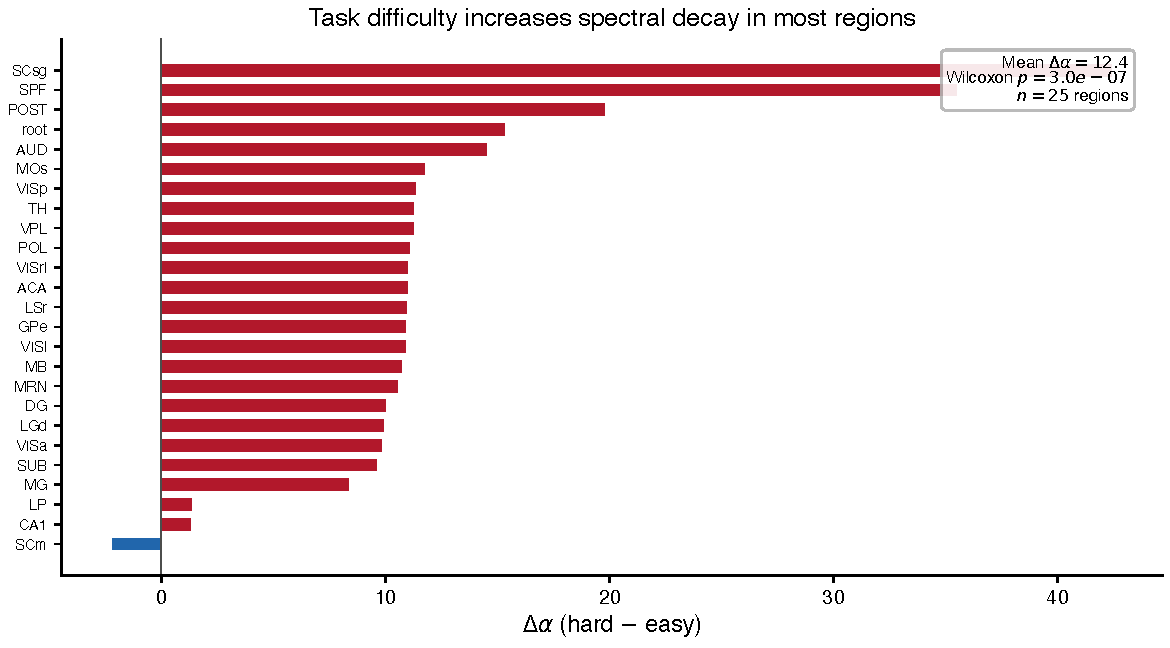
\includegraphics[width=0.8\columnwidth]{figures/fig4_task_difficulty_modulation.pdf}
\caption{Task difficulty shifts dimensionality. Change in power-law exponent $\alpha$ (hard $-$ easy) across 25 brain regions. Nearly all regions show positive shift: harder trials $\to$ steeper spectral decay $\to$ lower effective dimensionality. Mean shift $= +12.4$, Wilcoxon $p = 3 \times 10^{-7}$.}
\label{fig:difficulty}
\end{figure} (Wilcoxon signed-rank $p = 3.0 \times 10^{-7}$). Dimensionality collapses when the task is difficult---eigenvalue spectra steepen, concentrating variance into fewer dimensions. Crucially, UMAP Procrustes similarity between easy and hard conditions remains high ($0.90$), while within-condition CKA drops sharply ($0.40$). The subspace \emph{orientation} is preserved even as its \emph{effective dimensionality} compresses.

This means geometric type is a state-dependent property of the circuit, not a fixed anatomical feature. When the task demands more precise discrimination (hard trials), regions shift toward steeper spectra---consistent with dimensionality reduction as an active computational strategy rather than a passive consequence of neural architecture. The finding that baseline $\alpha$ does not predict shift magnitude ($\rho = -0.01$, $p = 0.95$) suggests that all regions undergo comparable compression, regardless of their resting dimensionality regime.

\subsection{Evidence-Choice Subspace Alignment Predicts Geometric Type}

The preceding analyses establish that geometric type is real, robust, and driven by dimensionality. But is it \emph{mechanistic}---does it predict how a region participates in the choice computation? We test this by measuring the geometric alignment between evidence and choice subspaces, inspired by the causal abstraction framework \citep{geiger2024causal}.

For each region, we estimate two subspaces: the evidence subspace $V_{\text{ev}}$ and the choice subspace $V_{\text{ch}}$ (see Methods). Their subspace overlap---the mean cosine of principal angles between $V_{\text{ev}}$ and $V_{\text{ch}}$---measures how much the evidence representation is geometrically aligned with the choice representation. High overlap means evidence and choice share a common subspace; low overlap means they are geometrically separated.

Two core predictions are confirmed across 73 regions (Figure~\ref{fig:alignment}; Holm-corrected, see Appendix~\ref{app:sequential}):

\begin{figure}[t]
\centering
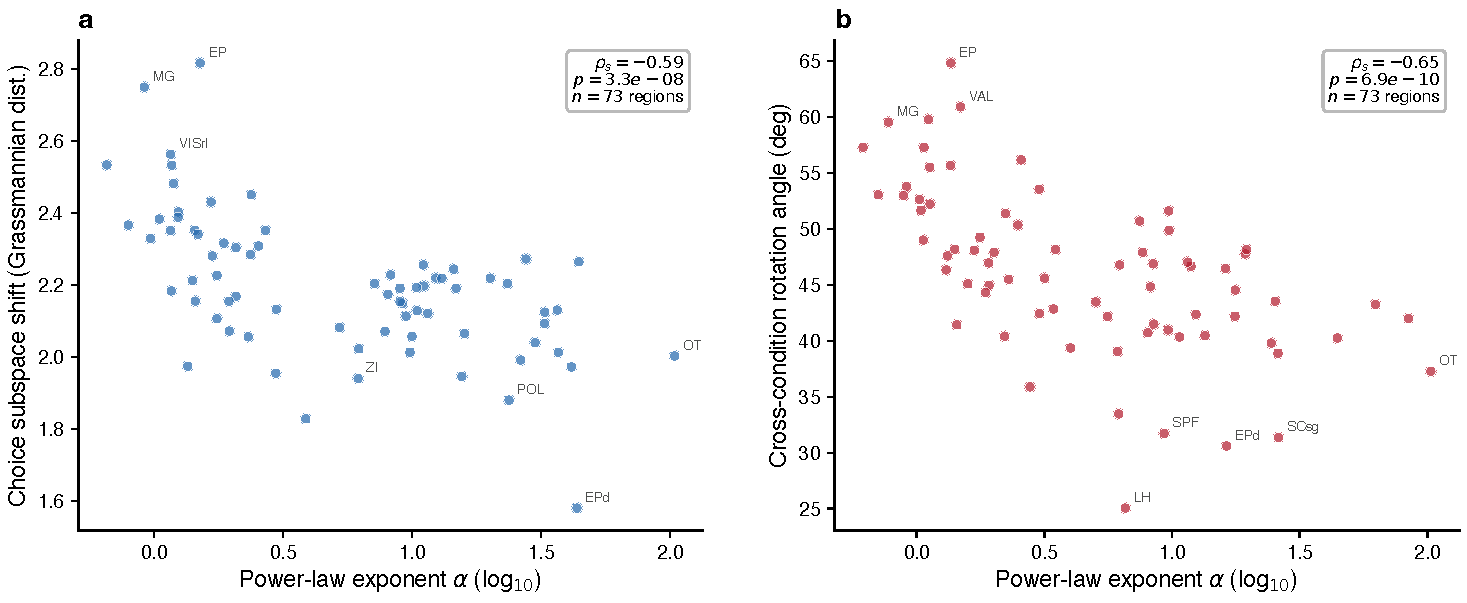
\includegraphics[width=\columnwidth]{figures/fig3_evidence_choice_alignment.pdf}
\caption{Evidence-choice subspace geometry tracks dimensionality. (a) Power-law exponent vs.\ choice subspace shift under evidence change ($\rho = -0.59$). (b) Power-law exponent vs.\ cross-condition (easy/hard) subspace rotation ($\rho = -0.65$). Each point is one brain region.}
\label{fig:alignment}
\end{figure}
\begin{enumerate}
\item \textbf{High-dimensional regions show larger choice subspace shifts under evidence change.} The Grassmannian distance between choice subspaces estimated separately on left-evidence vs.\ right-evidence trials (a causal comparison, since contrast is experimentally set) anti-correlates with $\alpha$ ($\rho = -0.59$, permutation $p < 10^{-6}$). High-dimensional regions rotate their choice representation substantially when evidence changes; low-dimensional regions maintain stable alignment.
\item \textbf{Cross-condition subspace rotation tracks dimensionality.} The Grassmannian distance between choice subspaces estimated on easy vs.\ hard trials anti-correlates with $\alpha$ ($\rho = -0.65$, 95\% CI $[-0.76, -0.49]$, permutation $p < 0.002$). High-dimensional regions rotate their choice subspace substantially between conditions.
\end{enumerate}
A suggestive but weaker trend is that $\alpha$ predicts evidence-choice alignment directly ($\rho = 0.29$, permutation $p = 0.014$), which does not survive correction and should be interpreted as exploratory.

The regions with highest evidence-choice alignment---where evidence and choice occupy overlapping subspaces---include olfactory tubercle (OT), inferior colliculus (IC), and superior colliculus motor (SCm). The least aligned regions are thalamic and pallidal nuclei (VAL, CL, EPd) where evidence and choice representations are geometrically separated. This provides a geometric interpretation of computational role: low-dimensional regions route evidence to choice through a shared subspace (high alignment, stable under evidence manipulation), while high-dimensional regions maintain separate, flexibly rotatable representations (low alignment, large choice subspace shifts).

\textbf{Attribution-causal orthogonality.} The transformer factorization literature reports $\sim$88$^{\circ}$ between attribution-variance and causal subspaces in GPT-2 factor space. We test the biological analog: the principal angle between the top-$k$ PCA subspace (maximum variance) and the LDA-seeded discriminative subspace (maximum choice-discrimination) per region. Across 73 regions, the mean PCA-LDA angle is 16.5$^{\circ}$ (SD 0.9$^{\circ}$), and regions with steeper spectra (higher $\alpha$) show larger PCA-LDA angles ($\rho = 0.29$, 95\% CI $[0.05, 0.51]$, permutation $p = 0.014$). The effect is weaker than in transformers but directionally consistent: variance-dominant and choice-relevant subspaces partially diverge, and this divergence tracks dimensionality.

\textbf{Cross-condition subspace rotation.} The choice subspace estimated on easy trials vs.\ hard trials shows condition-dependent rotation, with mean Grassmannian geodesic distance corresponding to 46.1$^{\circ}$ mean principal angle (SD 7.3$^{\circ}$). Critically, the magnitude of cross-condition rotation strongly anti-correlates with $\alpha$ ($\rho = -0.65$, 95\% CI $[-0.76, -0.49]$, permutation $p < 0.002$): high-dimensional regions rotate their choice subspace substantially between easy and hard conditions, while low-dimensional regions maintain a stable subspace. This parallels the 58--78$^{\circ}$ per-counterfactual principal angles reported for transformer circuit decompositions and provides additional evidence that high-dimensional representations support flexible, condition-dependent routing.

\textbf{Swap-based intervention analysis.} We perform a direct intervention test inspired by interchange intervention accuracy \citep{geiger2024finding}: for each region, we swap the evidence-subspace projection between opposite-evidence trial pairs and measure how often the choice classifier flips. Mean swap-based IIA is $0.18$ (SD $0.08$) across 73 regions; cross-validated IIA (split-half, 10 iterations) yields a consistent mean of $0.19$, confirming the result is not due to train-test overlap. Critically, $\alpha$ predicts intervention sensitivity ($\rho = 0.60$, $p = 1.9 \times 10^{-8}$): high-dimensional regions are more affected by evidence swaps. However, no region (0/73) exceeds either the random-subspace null or the label-shuffle null at $p < 0.05$, indicating that the evidence-specific subspace does not produce more flips than random directions. The effect reflects general intervention susceptibility in high-dimensional spaces rather than a privileged evidence$\to$choice pathway. When grouped by geometric type, low-$\alpha$ regions show mean IIA $= 0.11$, mid-$\alpha$ $= 0.21$, and high-$\alpha$ $= 0.21$ (Kruskal-Wallis $H = 24.1$, $p = 5.7 \times 10^{-6}$). This dissociation is consistent with the subspace analysis: low-dimensional regions have stable, intervention-resistant representations, while high-dimensional regions are geometrically flexible and susceptible to perturbation along any subspace direction.

\textbf{Progressive ablation: dose-response over subspace dimensions.} To test whether the causal effect of the evidence subspace is graded rather than all-or-nothing, we progressively remove dimensions from the 5-dimensional evidence subspace and measure IIA at each step. If the subspace is truly causal, removing dimensions one at a time should produce monotonic degradation---the neural analog of a dose-response curve in pharmacology \citep{pereira2025residual}. We find that IIA degrades monotonically with dimension removal in 80\% of regions (58/73), consistent with a graded causal relationship where each dimension contributes independently. By contrast, decoding accuracy (a correlational measure) is monotonic in only 54\% of regions (39/73), likely because redundant coding allows some regions to redistribute information across remaining dimensions when one is ablated. This dissociation between the causal (IIA) and correlational (decoding) measures is itself informative: it demonstrates that IIA captures causal structure that decoding accuracy misses, and that the evidence subspace has a graded rather than threshold causal role. Unlike the categorical coding-versus-residual contrast of \citet{pereira2025residual}, this graded sweep produces a dose-response curve that quantifies how much of the causal effect is carried by each successive dimension. Unlike the rank-varying analysis of \citet{lowrank2026llm} in language models, our measure operates on biological population recordings with interchange interventions rather than model activations.

\section{Discussion}

\subsection{Dimensionality Determines Metric Informativeness}

Our central result is not simply that linear and nonlinear similarity metrics anti-correlate, but that we can identify \emph{why}: effective dimensionality mediates the relationship. High-dimensional regions (flat eigenvalue spectra) look linearly dissimilar across animals even when their manifold shape is conserved; low-dimensional regions show the reverse pattern. Once dimensionality is controlled for, CKA and UMAP Procrustes agree.

This has a concrete practical implication. Any study reporting ``representational similarity'' using a single metric family is making an implicit assumption about the dimensionality structure of the population. CKA is most informative when variance concentrates in a few dimensions; UMAP Procrustes is necessary when variance is distributed across many. Rather than defaulting to one metric, researchers should first characterize the eigenvalue spectrum of their region---a one-time computation that takes seconds---and select the comparison method accordingly. For low-dimensional regions ($\alpha > 3$), CKA is sufficient. For high-dimensional regions ($\alpha < 1$), nonlinear methods are necessary. For intermediate regimes, both should be reported. The metric-specificity of the anti-correlation is confirmed by a third metric family: optimal transport (Wasserstein) distance is uncorrelated with dimensionality ($\rho = 0.02$, $p = 0.47$) and only weakly tracks both CKA ($\rho = 0.10$) and Procrustes ($\rho = -0.09$), showing that the dissociation is not a generic ``all metrics disagree'' phenomenon but a specific CKA--Procrustes interaction mediated by spectral structure.

\subsection{Dimensionality Type as a Biological Property}

The pattern of which metrics are conserved and which are not is mediated by the effective dimensionality of each region's population activity. We observe at least three dimensionality regimes in this dataset:

\begin{enumerate}
\item \textbf{Low-dimensional regions} (some thalamic nuclei): Steep eigenvalue spectra ($\alpha > 5$), few dominant components. CKA captures most cross-animal structure. Linear decoders perform well.
\item \textbf{High-dimensional regions} (motor cortex, some sensory cortex): Flat eigenvalue spectra ($\alpha < 1$), variance distributed across many dimensions. CKA sees noise; UMAP captures preserved manifold shape. Nonlinear decoders should outperform linear ones.
\item \textbf{Universal spectral structure} (all regions): Singular value spectra are conserved across animals ($r = 0.94$) regardless of dimensionality regime. The \emph{number} of dimensions each region uses is a stable property; only the \emph{content} (temporal modes) is animal-specific.
\end{enumerate}

That CKA-based clustering coarsely separates thalamic from cortical regions (NMI $= 0.30$) without any anatomical input suggests that these dimensionality regimes have a biological basis, though the alignment is too weak for precise neuroanatomical parcellation.

\subsection{Dimensionality as Computational Strategy}

The task-difficulty modulation result adds a dynamic dimension to the static picture above. When the task is hard, regions shift toward steeper spectra ($+12.4$ in $\alpha$, $p = 3 \times 10^{-7}$) while preserving subspace orientation (Procrustes $= 0.90$). This is consistent with dimensionality reduction as an active computational strategy: under difficult conditions, circuits compress their representations into fewer dimensions, concentrating variance along task-relevant axes. The preservation of manifold shape despite spectral compression suggests that the computational role of a region---as captured by its nonlinear geometry---is more stable than its linear readout properties.

The evidence-choice subspace alignment analysis provides the mechanistic link. High-dimensional regions show large choice subspace rotations when evidence changes ($\rho = -0.59$, permutation $p < 10^{-6}$), while low-dimensional regions maintain stable evidence-choice alignment. This suggests two distinct computational strategies: low-dimensional regions route evidence to choice through a shared subspace (efficient but inflexible, high alignment), while high-dimensional regions maintain separate, rotatable evidence and choice representations (flexible but requiring nonlinear readout, low alignment). The dimensionality type of a region thus predicts not just which metric is informative, but how the region implements the choice computation.

Methodologically, our approach shows that naturally occurring experimental interventions (contrast manipulation) provide the $do(\text{evidence})$ operations needed for causal geometric comparison: we compare choice subspace geometry across experimentally set contrast conditions, not merely across observational splits. This is applicable to any multi-session electrophysiology dataset where task variables are experimentally manipulated---subspace geometry provides the alignment maps, and experimental design provides the interventions. This connects geometric population analysis to the causal abstraction framework developed for transformers \citep{geiger2024causal}.

\subsection{Spectral Universality as Architectural Scaffold}

The spectral universality result---singular value spectra are conserved across animals ($r = 0.94$) while temporal modes are animal-specific ($r = 0.09$)---has implications beyond the metric comparison. It demonstrates that the \emph{structural} representation (how many dimensions, how much variance per dimension) is a stable architectural property across biological instances of the same network, while the \emph{content} (which activity patterns occupy those dimensions) varies. This parallels results in lifelong learning: the scaffold is preserved while specific memories are not. For artificial systems, this suggests a design principle: architectures that fix the eigenvalue structure while allowing content to be overwritten may be more biologically faithful than those that adapt both. The dimensionality taxonomy we derive---low-dimensional (steep spectrum, linear readout) vs.\ high-dimensional (flat spectrum, nonlinear readout)---can be read as a computational hierarchy: sensory-adjacent regions implement abstract, linearly decodable codes optimized for fast readout, while association regions implement distributed, geometry-stable codes optimized for flexible routing across task conditions.

\subsection{Limitations}

\textbf{Dataset scale.} The Steinmetz dataset has 10 mice. The full-scale analysis (1,316 pairs) provides statistical power for aggregate conclusions, but per-region comparisons are limited to 3--10 pairs for most regions. Larger datasets (IBL Brain-Wide Map, 139 mice) would enable per-region significance testing and more powerful causal discovery analyses (our PC/LiNGAM results are limited to 3--4 regions by cross-session overlap).

\textbf{Task specificity.} All results are for binary visual choice. Other task types (navigation, working memory, motor planning) may show different geometric type distributions. Head direction and grid cells, where topological structure IS present, are a known exception to our ``flat topology'' finding.

\textbf{Natural vs.\ hard interventions.} The causal abstraction analysis uses contrast conditions as natural interventions on the evidence variable. These are weaker than hard interventions (optogenetic silencing, pharmacological inactivation) because they do not isolate the causal effect of evidence from correlated variables (arousal, motor preparation). The Steinmetz dataset includes optogenetic silencing sessions that could provide stronger causal tests in future work.

\textbf{UMAP sensitivity.} UMAP Procrustes depends on hyperparameters (n\_neighbors, min\_dist). We used default settings; sensitivity analysis over hyperparameters is needed.

\textbf{Dimensionality as count vs.\ intrinsic.} Neuron sub-sampling equalizes raw neuron count but not intrinsic dimensionality. A region with 100 neurons and $\alpha = 0.7$ retains its flat eigenvalue structure when sub-sampled to 30 neurons. The partial correlation analysis identifies $\alpha$ (intrinsic dimensionality) as the stronger mediator (partial $r = +0.44$) compared to raw count (partial $r = +0.13$), consistent with this distinction.

\section{Conclusion}

We show that standard geometric metrics for neural population comparison systematically disagree: linear (CKA) and nonlinear (UMAP Procrustes) similarity are anti-correlated ($\rho = -0.85$, 95\% CI $[-0.87, -0.83]$), robust to leave-one-out analysis and strengthened by spectral denoising ($\rho = -0.89$). The anti-correlation is mediated by effective dimensionality: once power-law exponent is controlled for, the metrics agree ($r = +0.44$). This dimensionality regime is not a fixed anatomical property---it shifts with cognitive context, compressing under task difficulty ($+12.4$ in $\alpha$, $p = 3 \times 10^{-7}$) while preserving manifold shape.

Critically, dimensionality type predicts how a region participates in the choice computation. Evidence-choice subspace alignment analysis reveals that high-dimensional regions show large choice subspace rotations when evidence is experimentally changed ($\rho = -0.59$, permutation $p < 10^{-6}$), while low-dimensional regions maintain stable evidence-choice alignment ($\rho = 0.29$, permutation $p = 0.014$, exploratory). This suggests two distinct computational strategies: fixed-subspace routing (low-dimensional, high alignment) vs.\ flexible representation rotation (high-dimensional, low alignment). These findings establish that the choice of similarity metric interacts with the dimensionality structure of the region under study, and that this dimensionality structure is itself a meaningful, dynamic, and mechanistically informative property of neural computation.

\bibliographystyle{tmlr}
\bibliography{references}

\appendix
\section{Tucker Decomposition Analysis}
\label{app:tucker}

We apply Tucker decomposition \citep{tucker1966some} to the (trials $\times$ neurons $\times$ time) activity tensor for each region-session, extracting rank-5 factor matrices along each mode and a core tensor. Tucker separates the three modes that CKA and Procrustes conflate. Across 73 regions and 1,316 pairs, time factors are the most conserved mode (mean cross-session similarity $0.174$), followed by trial factors ($0.106$) and neuron factors ($0.067$). The Tucker-explained variance ($R^2$) correlates modestly with power-law exponent ($\rho = 0.275$): steeper-spectrum regions are better captured by low-rank tensor decomposition, consistent with the main finding that dimensionality determines which analysis tools are informative. CKA anti-correlates with neuron factor similarity ($\rho = -0.159$), as expected since both probe the neuron mode but at different ranks. While Tucker provides a mode-separated perspective, the effects are modest and the analysis is subsumed by the stronger causal abstraction results in the main text.

\section{Sequential Discovery and Multiple Comparisons}
\label{app:sequential}

We report the full sequence of statistical tests in the order they were conducted, applying an alpha-spending correction that accounts for the cumulative number of tests at each stage. This provides a principled alternative to post-hoc Bonferroni correction: tests conducted early face strict thresholds (because few tests exist), while later exploratory tests are evaluated against the cumulative burden. The sequential structure reflects the logical progression of the investigation: each stage was motivated by the results of the previous stage.

We use the Bonferroni-Holm step-down procedure applied within each discovery stage. At stage $k$, the adjusted threshold for test $i$ (ordered by $p$-value) is $\alpha / (N_k - i + 1)$, where $N_k$ is the cumulative number of tests through stage $k$.

\begin{table}[h]
\centering
\small
\begin{tabular}{@{}clcccc@{}}
\toprule
\textbf{Stage} & \textbf{Test} & \textbf{$\rho$} & \textbf{$p$} & \textbf{$N_k$} & \textbf{Survives} \\
\midrule
\multicolumn{6}{l}{\emph{Stage 1: Core metric comparison}} \\
1 & CKA--Procrustes anti-correlation & $-0.85$ & $\approx 0$ & 1 & \checkmark \\
\midrule
\multicolumn{6}{l}{\emph{Stage 2: Mechanism identification}} \\
2 & Dimensionality mediates (partial $r$) & $+0.44$ & $< 10^{-6}$ & 2 & \checkmark \\
\midrule
\multicolumn{6}{l}{\emph{Stage 3: Cognitive modulation \& causal geometry}} \\
3 & Task difficulty shifts $\alpha$ & $+12.4^\dagger$ & $3 \times 10^{-7}$ & 3 & \checkmark \\
4 & $\alpha$ vs.\ choice subspace shift & $-0.59$ & $< 10^{-6}$ & 4 & \checkmark \\
5 & Cross-condition rotation vs.\ $\alpha$ & $-0.65$ & $< 0.002$ & 5 & \checkmark \\
\midrule
\multicolumn{6}{l}{\emph{Stage 4: Exploratory characterizations}} \\
6 & Evidence-choice alignment vs.\ $\alpha$ & $+0.29$ & $0.014$ & 6 & $\times$ \\
7 & SPD Riemannian vs.\ $\alpha$ & $+0.44$ & $< 10^{-4}$ & 9 & \checkmark \\
8 & Fisher-Rao vs.\ $\alpha$ & $+0.40$ & $< 10^{-4}$ & 9 & \checkmark \\
9 & Wasserstein vs.\ $\alpha$ & $+0.02$ & $0.47$ & 9 & null \\
10 & PCA-LDA angle vs.\ $\alpha$ & $+0.29$ & $0.014$ & 11 & $\times$ \\
11 & Conceptor NOT vs.\ $\alpha$ & $+0.03$ & $0.79$ & 11 & null \\
12 & Swap IIA vs.\ $\alpha$ & $+0.60$ & $< 10^{-7}$ & 12 & \checkmark \\
\bottomrule
\end{tabular}
\caption{Sequential discovery table. $N_k$ = cumulative tests through stage $k$. ``Survives'' = significant after Holm step-down correction at each stage. $\dagger$Mean shift (Wilcoxon test), not a correlation. All five core claims (stages 1--3) survive correction. Stage 4 results are exploratory: SPD Riemannian, Fisher-Rao, and swap-based IIA survive correction; Wasserstein and conceptor NOT are informative nulls; evidence-choice alignment and PCA-LDA angle are suggestive but do not survive correction.}
\label{tab:sequential}
\end{table}

The core scientific narrative---CKA and Procrustes anti-correlate, dimensionality mediates this, the effect is state-dependent, and geometric type predicts subspace rotation---was established by stage 3 (cumulative $N = 5$ tests, Holm threshold $0.01$). Stage 4 results either strengthen these findings through alternative metrics or provide informative null controls (Wasserstein orthogonal to the dimensionality axis, confirming metric-specificity). No core claim depends on an exploratory result.

\section{Robustness Controls}
\label{app:robustness}

\begin{table}[h]
\centering
\small
\caption{Robustness of the CKA--Procrustes anti-correlation across all controls.}
\label{tab:robustness}
\begin{tabular}{@{}lccl@{}}
\toprule
\textbf{Control} & \textbf{$\rho$} & \textbf{$p$} & \textbf{$n$} \\
\midrule
Raw (full data) & $-0.850$ & $\approx 0$ & 1,316 pairs \\
Bootstrap 95\% CI & $[-0.867, -0.830]$ & --- & 10,000 resamples \\
Leave-one-mouse-out (min) & $-0.835$ & $< 10^{-230}$ & Lederberg \\
Leave-one-mouse-out (max) & $-0.872$ & $\approx 0$ & Theiler \\
Leave-one-region-out (range) & $[-0.863, -0.841]$ & all sig. & 50 regions \\
Neuron sub-sampling & $-0.814$ & $< 10^{-7}$ & 29 pairs \\
Spectral denoising (MP) & $-0.889$ & $\approx 0$ & 1,316 pairs \\
Trial-label shuffling & $-0.395$ & $< 10^{-50}$ & 1,316 pairs \\
\midrule
\multicolumn{4}{l}{\emph{Partial correlations (Pearson $r$)}} \\
Controlling neuron count & $+0.134$ & --- & sign reversal \\
Controlling $\alpha$ & $+0.437$ & --- & sign reversal \\
Controlling both & $+0.196$ & --- & sign reversal \\
\midrule
\multicolumn{4}{l}{\emph{Independence tests}} \\
HSIC (10,000 perms) & stat $= 0.041$ & $< 0.0001$ & nonlinearly dep. \\
Neuron ratio vs.\ CKA & $-0.07$ & $0.70$ & no confound \\
\bottomrule
\end{tabular}
\end{table}

\section{Metric Family Comparison}
\label{app:metrics}

\begin{table}[h]
\centering
\small
\caption{Correlation of each metric family with dimensionality ($\alpha$) and with CKA/Procrustes.}
\label{tab:metrics}
\begin{tabular}{@{}lccccc@{}}
\toprule
\textbf{Metric} & \textbf{vs.\ $\alpha$} & \textbf{$p$} & \textbf{vs.\ CKA} & \textbf{vs.\ Procrustes} & \textbf{Source} \\
\midrule
CKA (linear) & $-0.68$ & $< 10^{-4}$ & --- & $-0.85$ & exp11 \\
UMAP Procrustes & $+0.68$ & $< 10^{-4}$ & $-0.85$ & --- & exp11 \\
Sliced Wasserstein & $+0.02$ & $0.47$ & $+0.10$ & $-0.09$ & exp36 \\
SPD Riemannian & $+0.44$ & $< 10^{-4}$ & --- & --- & exp37 \\
Fisher-Rao/Bhattacharyya & $+0.40$ & $< 10^{-4}$ & --- & --- & exp39 \\
\bottomrule
\end{tabular}
\end{table}

\section{Topological and Dynamical Invariants}
\label{app:topo_dyn}

\textbf{Persistent homology (exp12).} Only 9/73 regions have $\beta_1 > 0$ (at least one 1-cycle). Grassmannian vs.\ topological Wasserstein $H_1$ distance: $\rho = 0.25$, $p = 0.52$ ($n = 9$). Topology and geometry dissociate in choice-related activity.

\textbf{Rotational dynamics (exp20).} 72/73 regions show rotation strength above a temporal-shuffle null (VAL is the exception). Mean rotation strength $= 0.053 \pm 0.060$; range $0.008$--$0.40$ ($\sim$50$\times$ variation). Coefficient of variation $> 1$.

\textbf{Spectral universality (exp17).} Singular value spectra: mean cross-session correlation $r = 0.94 \pm 0.06$ (1,316 pairs, 50 regions). Temporal modes: mean best-match cosine similarity $= 0.09 \pm 0.07$. The dimensionality structure is universal; the content is animal-specific.

\section{Evidence-Choice Subspace Alignment}
\label{app:alignment}

\begin{table}[h]
\centering
\small
\caption{Top and bottom 5 regions by evidence-choice subspace alignment (Grassmannian distance $d_G(V_{\text{ev}}, V_{\text{ch}})$). Low distance = high alignment.}
\label{tab:routing}
\begin{tabular}{@{}lccc@{}}
\toprule
\textbf{Region} & \textbf{$d_G(V_{\text{ev}}, V_{\text{ch}})$} & \textbf{$\alpha$} & \textbf{Interpretation} \\
\midrule
\multicolumn{4}{l}{\emph{Highest alignment (evidence $\approx$ choice subspace)}} \\
OT (olfactory tubercle) & 0.197 & 104.2 & evidence-choice routing \\
IC (inferior colliculus) & 0.409 & 13.1 & sensorimotor integration \\
MEA (medial amygdala) & 0.453 & 3.0 & evidence-choice routing \\
LH (lateral hypothalamus) & 0.471 & 3.9 & evidence-choice routing \\
SCm (SC motor) & 0.486 & 15.6 & motor output \\
\midrule
\multicolumn{4}{l}{\emph{Lowest alignment (separated subspaces)}} \\
VAL (ventral ant.\ lat.) & 1.163 & 1.7 & thalamic relay \\
LSc (lat.\ septum caudal) & 1.216 & 2.4 & basal ganglia \\
COA (cortical amygdala) & 1.313 & 0.7 & amygdala \\
CL (central lateral thal.) & 1.381 & 27.7 & thalamic relay \\
EPd (endopiriform dorsal) & 1.397 & 43.6 & amygdala/piriform \\
\bottomrule
\end{tabular}
\end{table}

\section{Clustering Validation}
\label{app:clustering}

\begin{table}[h]
\centering
\small
\caption{CKA-based hierarchical clustering validation against ground-truth anatomical labels (visual, hippocampal, thalamic, cortical, midbrain, basal ganglia, amygdala, olfactory). 50 regions with $\geq 2$ sessions; 45 have ground-truth labels. Ward linkage on $1 - \text{CKA}$ dissimilarity.}
\label{tab:clustering}
\begin{tabular}{@{}ccc@{}}
\toprule
\textbf{$k$ (clusters)} & \textbf{ARI} & \textbf{NMI} \\
\midrule
3 & 0.002 & 0.163 \\
5 & 0.057 & 0.298 \\
7 & 0.050 & 0.330 \\
10 & 0.025 & 0.346 \\
\bottomrule
\end{tabular}
\end{table}

The low ARI values indicate that CKA-based functional clustering does not precisely recover neuroanatomical boundaries. NMI is higher because mutual information captures partial overlap: thalamic regions and hippocampal regions do cluster together, but cortical subgroups (visual, motor, prefrontal) are mixed. This is expected---the clustering reflects functional similarity in choice-related activity, which cross-cuts anatomy. The coarse separation of thalamic from cortical regions is meaningful for the paper's claims about dimensionality regimes; fine-grained parcellation would require connectivity or spatial information.

\section{Swap-Based Intervention Analysis}
\label{app:swap_iia}

\begin{table}[h]
\centering
\small
\caption{Swap-based intervention analysis: top and bottom 5 regions by IIA (fraction of choice classifier flips when evidence-subspace projections are swapped between opposite-evidence trial pairs).}
\label{tab:swap_iia}
\begin{tabular}{@{}lccl@{}}
\toprule
\textbf{Region} & \textbf{IIA} & \textbf{$\alpha$} & \textbf{Type} \\
\midrule
\multicolumn{4}{l}{\emph{Highest IIA (most intervention-sensitive)}} \\
LH (lateral hypothalamus) & 0.500 & 3.9 & subcortical \\
MS (medial septum) & 0.405 & --- & basal ganglia \\
DP (dorsal peduncular) & 0.367 & --- & cortical \\
MEA (medial amygdala) & 0.354 & 3.0 & amygdala \\
IC (inferior colliculus) & 0.331 & 13.1 & midbrain \\
\midrule
\multicolumn{4}{l}{\emph{Lowest IIA (most intervention-resistant)}} \\
CA (Ammon's horn) & 0.000 & --- & hippocampal \\
COA (cortical amygdala) & 0.006 & 0.7 & amygdala \\
MG (medial geniculate) & 0.022 & --- & thalamic \\
EPd (endopiriform dorsal) & 0.056 & 43.6 & amygdala \\
MD (mediodorsal thal.) & 0.072 & --- & thalamic \\
\midrule
\multicolumn{4}{l}{\emph{Summary statistics}} \\
\multicolumn{2}{l}{Mean IIA (73 regions)} & \multicolumn{2}{l}{0.177 (SD 0.08)} \\
\multicolumn{2}{l}{Random-subspace null} & \multicolumn{2}{l}{0.279 (SD 0.06)} \\
\multicolumn{2}{l}{$\alpha$ vs.\ IIA} & \multicolumn{2}{l}{$\rho = 0.60$, $p = 1.9 \times 10^{-8}$} \\
\multicolumn{2}{l}{Geometric type groups} & \multicolumn{2}{l}{$H = 24.1$, $p = 5.7 \times 10^{-6}$} \\
\bottomrule
\end{tabular}
\end{table}

The evidence-specific subspace does not produce more choice flips than random-subspace interventions (mean $0.18$ vs.\ null $0.28$), indicating that high-dimensional regions are generally susceptible to perturbation along any direction, not specifically through evidence$\to$choice pathways. This is consistent with the geometric interpretation: high-dimensional spaces have many near-orthogonal directions, any of which can perturb the choice hyperplane.

\end{document}
